\documentclass{standalone}
\usepackage{tikz}
\usetikzlibrary{patterns, positioning}


\begin{document}
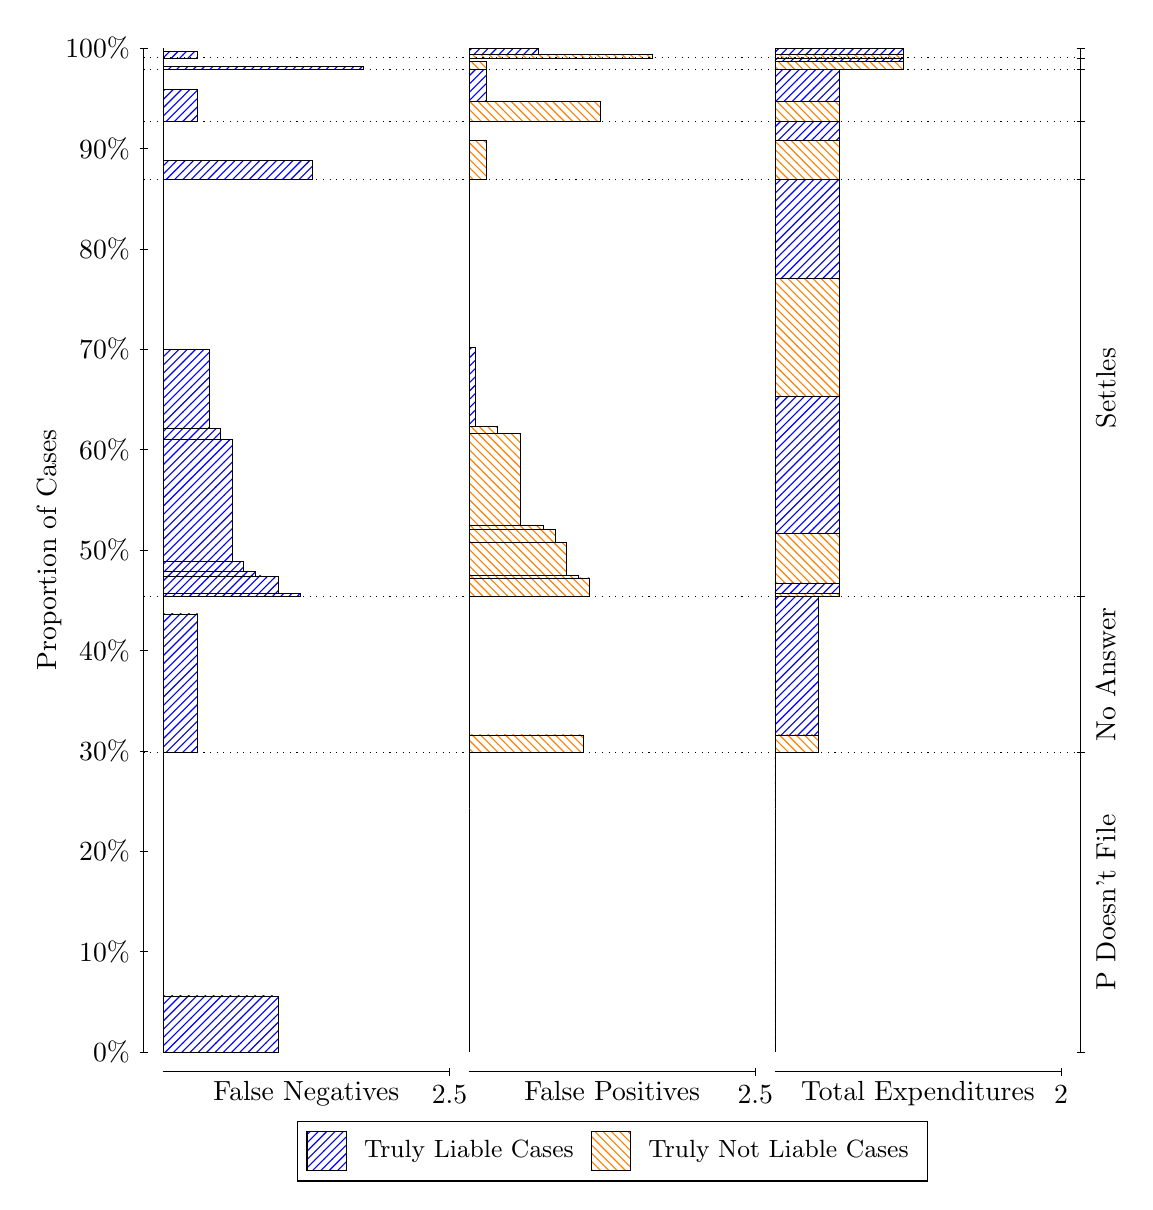
\begin{tikzpicture}
\draw[black, very thin] (1.5,1.75) -- (1.5,14.5);
\node[rotate=90, text=black, anchor=center] at (0.3, 8.125) {Proportion of Cases};
\draw[black, very thin] (1.45,1.75) -- (1.55,1.75);
\node[text=black, anchor=east] at (1.45, 1.75) {0\%};
\draw[black, very thin] (1.45,3.025) -- (1.55,3.025);
\node[text=black, anchor=east] at (1.45, 3.025) {10\%};
\draw[black, very thin] (1.45,4.3) -- (1.55,4.3);
\node[text=black, anchor=east] at (1.45, 4.3) {20\%};
\draw[black, very thin] (1.45,5.575) -- (1.55,5.575);
\node[text=black, anchor=east] at (1.45, 5.575) {30\%};
\draw[black, very thin] (1.45,6.85) -- (1.55,6.85);
\node[text=black, anchor=east] at (1.45, 6.85) {40\%};
\draw[black, very thin] (1.45,8.125) -- (1.55,8.125);
\node[text=black, anchor=east] at (1.45, 8.125) {50\%};
\draw[black, very thin] (1.45,9.4) -- (1.55,9.4);
\node[text=black, anchor=east] at (1.45, 9.4) {60\%};
\draw[black, very thin] (1.45,10.675) -- (1.55,10.675);
\node[text=black, anchor=east] at (1.45, 10.675) {70\%};
\draw[black, very thin] (1.45,11.95) -- (1.55,11.95);
\node[text=black, anchor=east] at (1.45, 11.95) {80\%};
\draw[black, very thin] (1.45,13.225) -- (1.55,13.225);
\node[text=black, anchor=east] at (1.45, 13.225) {90\%};
\draw[black, very thin] (1.45,14.5) -- (1.55,14.5);
\node[text=black, anchor=east] at (1.45, 14.5) {100\%};

\draw[black, very thin] (13.4,1.75) -- (13.4,14.5);
\draw[black, very thin] (13.35,1.75) -- (13.45,1.75);
\node[anchor=west] at (13.35, 1.75) {};
\draw[black, very thin] (13.35,5.5528) -- (13.45,5.5528);
\node[anchor=west] at (13.35, 5.5528) {};
\draw[black, very thin] (13.35,7.538) -- (13.45,7.538);
\node[anchor=west] at (13.35, 7.538) {};
\draw[black, very thin] (13.35,12.828) -- (13.45,12.828);
\node[anchor=west] at (13.35, 12.828) {};
\draw[black, very thin] (13.35,13.566) -- (13.45,13.566);
\node[anchor=west] at (13.35, 13.566) {};
\draw[black, very thin] (13.35,14.227) -- (13.45,14.227);
\node[anchor=west] at (13.35, 14.227) {};
\draw[black, very thin] (13.35,14.376) -- (13.45,14.376);
\node[anchor=west] at (13.35, 14.376) {};
\draw[black, very thin] (13.35,14.5) -- (13.45,14.5);
\node[anchor=west] at (13.35, 14.5) {};

\draw[black, very thin, pattern color=blue, pattern=north east lines] (1.75,1.75) rectangle (3.2033,2.4616);
\draw[black, very thin, pattern color=orange, pattern=north west lines] (1.75,2.4616) rectangle (1.75,5.5528);
\draw[black, very thin, pattern color=blue, pattern=north east lines] (1.75,5.5528) rectangle (2.186,7.3138);
\draw[black, very thin, pattern color=orange, pattern=north west lines] (1.75,7.3138) rectangle (1.75,7.538);
\draw[black, very thin, pattern color=blue, pattern=north east lines] (1.75,7.538) rectangle (3.494,7.5776);
\draw[black, very thin, pattern color=blue, pattern=north east lines] (1.75,7.5776) rectangle (3.2033,7.7925);
\draw[black, very thin, pattern color=blue, pattern=north east lines] (1.75,7.7925) rectangle (3.058,7.7956);
\draw[black, very thin, pattern color=blue, pattern=north east lines] (1.75,7.7956) rectangle (2.9127,7.8488);
\draw[black, very thin, pattern color=blue, pattern=north east lines] (1.75,7.8488) rectangle (2.7673,7.9819);
\draw[black, very thin, pattern color=blue, pattern=north east lines] (1.75,7.9819) rectangle (2.622,9.5314);
\draw[black, very thin, pattern color=blue, pattern=north east lines] (1.75,9.5314) rectangle (2.4767,9.667);
\draw[black, very thin, pattern color=blue, pattern=north east lines] (1.75,9.667) rectangle (2.3313,10.668);
\draw[black, very thin, pattern color=orange, pattern=north west lines] (1.75,10.668) rectangle (1.75,12.828);
\draw[black, very thin, pattern color=blue, pattern=north east lines] (1.75,12.828) rectangle (3.6393,13.071);
\draw[black, very thin, pattern color=orange, pattern=north west lines] (1.75,13.071) rectangle (1.75,13.566);
\draw[black, very thin, pattern color=blue, pattern=north east lines] (1.75,13.566) rectangle (2.186,13.972);
\draw[black, very thin, pattern color=orange, pattern=north west lines] (1.75,13.972) rectangle (1.75,14.227);
\draw[black, very thin, pattern color=blue, pattern=north east lines] (1.75,14.227) rectangle (4.2933,14.269);
\draw[black, very thin, pattern color=orange, pattern=north west lines] (1.75,14.269) rectangle (1.75,14.376);
\draw[black, very thin, pattern color=blue, pattern=north east lines] (1.75,14.376) rectangle (2.186,14.457);
\draw[black, very thin, pattern color=orange, pattern=north west lines] (1.75,14.457) rectangle (1.75,14.5);
\draw[black, very thin, pattern color=orange, pattern=north west lines] (5.6333,1.75) rectangle (5.6333,4.8412);
\draw[black, very thin, pattern color=blue, pattern=north east lines] (5.6333,4.8412) rectangle (5.6333,5.5528);
\draw[black, very thin, pattern color=orange, pattern=north west lines] (5.6333,5.5528) rectangle (7.0867,5.777);
\draw[black, very thin, pattern color=blue, pattern=north east lines] (5.6333,5.777) rectangle (5.6333,7.538);
\draw[black, very thin, pattern color=orange, pattern=north west lines] (5.6333,7.538) rectangle (7.1593,7.7704);
\draw[black, very thin, pattern color=orange, pattern=north west lines] (5.6333,7.7704) rectangle (7.014,7.8048);
\draw[black, very thin, pattern color=orange, pattern=north west lines] (5.6333,7.8048) rectangle (6.8687,8.2261);
\draw[black, very thin, pattern color=orange, pattern=north west lines] (5.6333,8.2261) rectangle (6.7233,8.3911);
\draw[black, very thin, pattern color=orange, pattern=north west lines] (5.6333,8.3911) rectangle (6.578,8.4357);
\draw[black, very thin, pattern color=orange, pattern=north west lines] (5.6333,8.4357) rectangle (6.4327,8.4387);
\draw[black, very thin, pattern color=orange, pattern=north west lines] (5.6333,8.4387) rectangle (6.2873,9.6099);
\draw[black, very thin, pattern color=orange, pattern=north west lines] (5.6333,9.6099) rectangle (5.9967,9.6983);
\draw[black, very thin, pattern color=blue, pattern=north east lines] (5.6333,9.6983) rectangle (5.706,10.699);
\draw[black, very thin, pattern color=blue, pattern=north east lines] (5.6333,10.699) rectangle (5.6333,12.828);
\draw[black, very thin, pattern color=orange, pattern=north west lines] (5.6333,12.828) rectangle (5.8513,13.323);
\draw[black, very thin, pattern color=blue, pattern=north east lines] (5.6333,13.323) rectangle (5.6333,13.566);
\draw[black, very thin, pattern color=orange, pattern=north west lines] (5.6333,13.566) rectangle (7.3047,13.821);
\draw[black, very thin, pattern color=blue, pattern=north east lines] (5.6333,13.821) rectangle (5.8513,14.227);
\draw[black, very thin, pattern color=orange, pattern=north west lines] (5.6333,14.227) rectangle (5.8513,14.333);
\draw[black, very thin, pattern color=blue, pattern=north east lines] (5.6333,14.333) rectangle (5.6333,14.376);
\draw[black, very thin, pattern color=orange, pattern=north west lines] (5.6333,14.376) rectangle (7.9587,14.419);
\draw[black, very thin, pattern color=blue, pattern=north east lines] (5.6333,14.419) rectangle (6.5053,14.5);
\draw[black, very thin, pattern color=orange, pattern=north west lines] (9.5167,1.75) rectangle (9.5167,4.8412);
\draw[black, very thin, pattern color=blue, pattern=north east lines] (9.5167,4.8412) rectangle (9.5167,5.5528);
\draw[black, very thin, pattern color=orange, pattern=north west lines] (9.5167,5.5528) rectangle (10.062,5.777);
\draw[black, very thin, pattern color=blue, pattern=north east lines] (9.5167,5.777) rectangle (10.062,7.538);
\draw[black, very thin, pattern color=orange, pattern=north west lines] (9.5167,7.538) rectangle (10.334,7.5725);
\draw[black, very thin, pattern color=blue, pattern=north east lines] (9.5167,7.5725) rectangle (10.334,7.708);
\draw[black, very thin, pattern color=orange, pattern=north west lines] (9.5167,7.708) rectangle (10.334,8.3388);
\draw[black, very thin, pattern color=blue, pattern=north east lines] (9.5167,8.3388) rectangle (10.334,10.075);
\draw[black, very thin, pattern color=orange, pattern=north west lines] (9.5167,10.075) rectangle (10.334,11.57);
\draw[black, very thin, pattern color=blue, pattern=north east lines] (9.5167,11.57) rectangle (10.334,12.828);
\draw[black, very thin, pattern color=orange, pattern=north west lines] (9.5167,12.828) rectangle (10.334,13.323);
\draw[black, very thin, pattern color=blue, pattern=north east lines] (9.5167,13.323) rectangle (10.334,13.566);
\draw[black, very thin, pattern color=orange, pattern=north west lines] (9.5167,13.566) rectangle (10.334,13.821);
\draw[black, very thin, pattern color=blue, pattern=north east lines] (9.5167,13.821) rectangle (10.334,14.227);
\draw[black, very thin, pattern color=orange, pattern=north west lines] (9.5167,14.227) rectangle (11.152,14.333);
\draw[black, very thin, pattern color=blue, pattern=north east lines] (9.5167,14.333) rectangle (11.152,14.376);
\draw[black, very thin, pattern color=orange, pattern=north west lines] (9.5167,14.376) rectangle (11.152,14.419);
\draw[black, very thin, pattern color=blue, pattern=north east lines] (9.5167,14.419) rectangle (11.152,14.5);
\draw[black, dotted] (1.5,5.5528) -- (13.4,5.5528);
\draw[black, dotted] (1.5,7.538) -- (13.4,7.538);
\draw[black, dotted] (1.5,12.828) -- (13.4,12.828);
\draw[black, dotted] (1.5,13.566) -- (13.4,13.566);
\draw[black, dotted] (1.5,14.227) -- (13.4,14.227);
\draw[black, dotted] (1.5,14.376) -- (13.4,14.376);
\draw[black, very thin] (1.75,1.5) -- (5.3833,1.5);
\node[text=black, anchor=north] at (3.5667, 1.5) {False Negatives};
\draw[black, very thin] (5.3833,1.45) -- (5.3833,1.55);
\node[text=black, anchor=north] at (5.3833, 1.45) {2.5};

\draw[black, very thin] (5.6333,1.5) -- (9.2667,1.5);
\node[text=black, anchor=north] at (7.45, 1.5) {False Positives};
\draw[black, very thin] (9.2667,1.45) -- (9.2667,1.55);
\node[text=black, anchor=north] at (9.2667, 1.45) {2.5};

\draw[black, very thin] (9.5167,1.5) -- (13.15,1.5);
\node[text=black, anchor=north] at (11.333, 1.5) {Total Expenditures};
\draw[black, very thin] (13.15,1.45) -- (13.15,1.55);
\node[text=black, anchor=north] at (13.15, 1.45) {2};

\node[text=black, centered, rotate=90] at (13.72, 3.6514) {P Doesn't File};
\node[text=black, centered, rotate=90] at (13.72, 6.5454) {No Answer};
\node[text=black, centered, rotate=90] at (13.72, 10.183) {Settles};





\draw (7.449999999999999,1.5) node[draw=none] (baseCoordinate) {};
\begin{scope}[align=center]
        \matrix[scale=0.5, draw=black, below=0.5cm of baseCoordinate, nodes={draw}, column sep=0.1cm]{
            \node[rectangle, draw, minimum width=0.5cm, minimum height=0.5cm, pattern color=blue, pattern=north east lines] {}; &
            \node[draw=none, font=\small, text=black] (B) {Truly Liable Cases}; &
            \node[rectangle, draw, minimum width=0.5cm, minimum height=0.5cm, pattern color=orange, pattern=north west lines] {}; &
            \node[draw=none, font=\small, text=black] (B) {Truly Not Liable Cases}; \\
            };
\end{scope}

\end{tikzpicture}
\end{document}